\reportpage{05 / PHYSICS BEHIND THE PICTURES}{Reading the 3D simulation correctly}
A trajectory's appearance depends on the reference frame. The same planet follows a closed orbit in a co-moving view and a winding path when Solar travel is included. This does not imply a universal helix through spacetime.
\begin{center}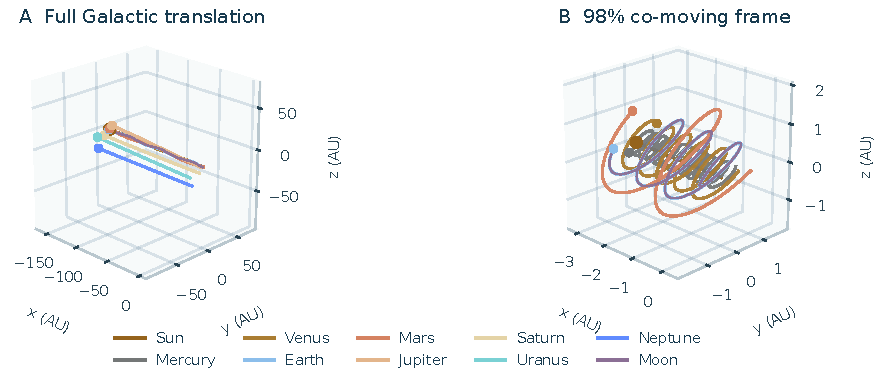
\includegraphics[width=\linewidth,height=67mm,keepaspectratio]{paths.pdf}\end{center}
\figcap{Three model years: A shows all ten bodies; B shows the Sun, inner planets and Moon. Each panel has equal AU axes with different displayed ranges. Markers are enlarged. Vector model plots, not website screenshots.}

\subsection*{Three motions that should not be confused}
\textbf{Planetary reflex:} the Sun moves around the Solar System barycentre in response to the planets. \textbf{Vertical Solar oscillation:} the long-clock orbit moves above and below the model Galactic midplane. \textbf{Galactic warp:} the displayed outer-disk bend is a separate kinematic illustration [8]. It does not supply an additional force to the Solar integration.

The long clock uses a nearly circular orbit in a static smooth potential. \textbf{A self-consistent evolution of the Galactic plane is not modelled.} The ecliptic's roughly $60^\circ$ tilt is relative to the Galactic plane; it is not the inclination of the Sun's entire Galactic orbit.

\begin{minipage}[t]{.485\linewidth}\vspace{0pt}\setlength{\parskip}{3pt}
\subsection*{A released probe keeps moving}
A passive probe inherits its release velocity and accelerates under gravity. Leaving it outside Earth does not leave it at a fixed Galactic coordinate.

The cyan 2026 marker is a \emph{hypothetical held reference}. Cancelling its velocity and holding it fixed would require a specified propulsion and force-compensation scheme. The simulation does not design such a mission.
\subsection*{The heliosphere is not a wall}
The model marks a 120 AU heliopause, a 90 AU termination shock and radial 400 km/s wind tracers inside the shock. Real boundaries are asymmetric and time dependent [9]; energetic cosmic rays can penetrate. No MHD or radiation-transport calculation is claimed.
\end{minipage}\hfill
\begin{minipage}[t]{.485\linewidth}\vspace{0pt}\setlength{\parskip}{3pt}
\subsection*{Gravity and clocks}
For an isolated, nonrotating spherical body, a held clock and an ideal circular-orbit clock satisfy
\begin{align}
 \left(\frac{d\tau}{dt}\right)_{\!\mathrm{held}}&=\sqrt{1-\frac{2GM}{rc^2}},\\
 \left(\frac{d\tau}{dt}\right)_{\!\mathrm{circular}}&=\sqrt{1-\frac{3GM}{rc^2}}.
\end{align}
Here $t$ refers to a clock at infinity. Relative to a stationary spherical-Earth surface clock, a circular clock loses \textbf{24.74 $\mu$s/day at 400 km} and gains \textbf{38.51 $\mu$s/day at 20,200 km} [10]. Rotation and operational corrections are excluded.

The whole-system view sums ten masses at a fixed test point using a weak-field clock rate. The potential sheet has arbitrary display depth.
\end{minipage}

\takeaway{A tested approximation, not full GR}{The separate coupled 1PN lab starts from JPL states [11]. Its two-body Mercury benchmark gives 42.9798 arcsec/century against 42.9807 analytically. The ten-year lunar discrepancy reaches 215 km. This is not a navigation ephemeris.}
